\chapter{COMPRESSING THE TENSOR INDICES}
    
        As we already discussed, sparsification is a compression method that can be used to reduce the size of gradients exchanged between workers.
        Out of the $d$ components that comprise a stochastic gradient we select only a subset of them to communicate to the network. 
        Let $r$ be the number of components that we choose to send, where $r<d$. 
        These $r$ elements can be selected via a variety of different methods 
        (e.g Top-r, Random-r etc) and the information they carry is strictly tied to their positions inside the initial gradient vector.
        Therefore, these positions must be conveyed as information to the workers alongside the values of the sparsified gradient.
        Only this way the workers receiving the message will be able to correctly perform the decompression process.
        However, a representation of these positions must now be employed and an idea that we entertain and explore the most, throughout this thesis, for achieving space-efficient representations is that of using bloom filters.
        We are also experimenting with a variety of more simple approaches that we eventually use as baselines for the bloom filter approach. 
        However, we will discuss those in a later chapter.

    \section{Encoding/Decoding}
        Let $g\in\R^d$ be the stochastic gradient and $\tilde{g}\in\R^d$ be the sparsified gradient with $\|\tilde{g}\|_0=r$. For distributed training, one has to send the tuple $(\tilde{g}[i],i)$, where $\tilde{g}[i]\neq 0$. Let $S$ be the set of $r$ indices corresponding to the sparsified gradient components  and we use a Bloom filter to send those indices. Note that, $S'$ would now be the set of all the rest $d-r$ indices that correspond to zero gradient values. The union of $S$ and $S'$ is finite and constitutes the universe $U$ of the bloom filter. Consider a bit string $\cS$ of $m$ bits all set to 0, initially. Let there be $k$ hash functions $h_i$, each of which hashes each index $i\in S$ and yields a bit-location in $\cS$ and changes the corresponding bit 0 at that bit-location to 1. We note that only the first bit-change in a location of $\cS$ has effect, that is, if a bit-location is already set to 1 from a previous hashing, any other changes at that bit-location due to consequent hashing have no effect. Finally, we send the modified bit array $\cS$ along with the set of nonzero gradient values $\{\tilde{g}[i]\}_{i\in S}$.
        For decompression, one needs to use membership queries for all the elements inside $U$ to check which of those (in our case, the indices of the sparsified gradient components) belong to the set of indices, $S$. To check whether an element $y_j$ belongs to the set of indices, $S$, one has to use $k$ hash functions on it. If $h_i(y_j)=0$ for any $i=1,2,\cdots,k$, then we {\em surely} know that element does not belong to $S$. On the other hand, if $h_i(y_j)=1$ for all $i=1,2,\cdots,k$, then that element may or may not belong to $S$. The querying process for a given element is described in Algorithm \ref{alg_1:query_BF}. Once the querying is done, a new set $P$ will be created containing all those elements that correspond to the non-negative responses. Our set $S$ is a subset of $P$ and the elements included there are the True Positive responses of the bloom filter. Consequently, $P-S$ contains all the False Positive ones. A policy must now be adopted for drawing $r$ elements from $P$. Ideally, we would want that policy to select the $r$ elements of our set $S$ and discard the false positive ones but this will rarely be the case under the existence of many false positives.
        For every index chosen a nonzero value from $\{\tilde{g}[i]\}_{i\in S}$ is assigned to reconstruct the sparse vector. For the rest of the indices inside $U$ we assign a zero value. Note that, the mapping between the nonzero values and the chosen indices is not arbitrary. As long as the given policy selects indices in a deterministic manner, we can ensure that the values in $\{\tilde{g}[i]\}_{i\in S}$ will be assigned in an optimal way. It is readily seen, however, that a completely correct reconstruction of the sparsified vector cannot be guaranteed under the current setting. That is because the selection of one or more indices corresponding to false positive responses will disrupt the mapping process and will cause re-arrangements and shifts of the reconstructed gradient components with respect to their true positions. The decompression process is described in Algorithm \ref{alg_3:decompress_BF}.
        
        \begin{figure}
        \begin{minipage}{1\textwidth}
        \centering
        \begin{algorithm}[H]
        	\SetAlgoLined
         	\SetKwInOut{Input}{Input}
        	\SetKwInOut{Output}{Output}
             \SetKwInOut{Init}{Initialize}
             \SetKwInOut{Compute}{Compute}
        \nl\Input{Bloom filter $\cB$, $k$-hash functions $h_i$, a set $U$, an empty set $P$, a policy $\mathcal{P}$, $r$, $\{\tilde{g}[i]\}_{i\in S}$;}
         \nl \For{each $y_j\in U$}
            {\nl Query the element $y_j$ using $\cS$ and the $k$-hash functions\;
            \nl \If{$y_j$ is in $\cS$}
        		    {\nl {\tt Insert $y_j$ in $P$}\;
        		}
         	}
           \nl {\tt Draw $r$ indices from $P$ using the policy $\mathcal{P}$}\;
            \nl \For{each $y_j\ in $ drawn indices}
            {\nl {\tt Assign a value from $\{\tilde{g}[i]\}_{i\in S}$ to the position $y_j$ of the reconstructed vector }\;
         	}
         	\nl \For{each $y_j$in $U-P$}
            {\nl {\tt Assign zero to the position $y_j$ of the reconstructed vector }\;
         	}
         	\caption{Decompressing a sparsified gradient by using Bloom filter} \label{alg_3:decompress_BF}
         \end{algorithm}
        \end{minipage}
        \end{figure}
    
    % \section{Tuning the bloom filter parameters}
    % \newpage

    \section{Tuning the Bloom Filter Parameters}

    Tuning appropriately the bloom filter parameters like its size $m$ or the number of hash functions $k$, is a matter of great importance.
    Those have an immediate impact to the bloom filter's performance both in terms of accuracy and throughput.
    In our bloom filter compression approach, we let the user define the false positive rate that suits their needs and the $m$ and $k$ parameters are automatically derived by the mathematical formulas \cite{5751342} we discussed in an earlier section.
    
    More specifically, given a false positive rate $\epsilon$, we define the bloom filter size as:
    \begin{flushleft}
    \centering
    \setlength{\parindent}{5ex}
    $m=\frac{-r\log\epsilon}{(\log 2)^2}$
    \end{flushleft} 
    and the number of hash functions as:
    \begin{flushleft}
    \centering
    \setlength{\parindent}{5ex}
    $k=\frac{-\log\epsilon}{\log 2}$
    \end{flushleft}
    
    \section{Reconstruction Errors}
            Representing the set $S$ using a Bloom Filter is more space-efficient compared to other approaches, however, the inevitable occurrence of false positive responses creates a variety of errors while reconstructing the sparsified gradient. In this section, we investigate the nature of these errors, as well as their actual impact on the reconstruction process.
            
            As we discussed earlier, $\{\tilde{g}[i]\}_{i\in S}$ denotes the sparsified gradient components that we wish to decode and $P$ is the set of elements from the universe $U$ that correspond to non-negative bloom filter responses.
            Let $\tilde{S}$ be the set of the $r$ indices selected from $P$ by a specified policy 
            $\mathcal{P}$. 
            One method to evaluate how good $\mathcal{P}$ is, would be to measure the similarity between $\tilde{S}$ and our true set of indices, $S$. 
            That is, to measure the number of elements by which those two sets differ. 
        
            For the decompression, we use a mapping $\mathcal{M}$ that assigns each element from $\tilde{S}$ to a unique element from $\{\tilde{g}[i]\}_{i\in S}$.
            It is only logical that $\mathcal{M}$ must at least guarantee a correct reconstruction under the complete absence of false positive responses. 
            We can choose a very simple mapping process that achieves the above, given the assumption that the values of the sparsified gradient are communicated through the network in a very specific order. 
            Note that, during the compression phase we have total control over the form of the message that is to be sent and therefore, the order of the values.
            That said, we make the convention that all values in $\{\tilde{g}[i]\}_{i\in S}$ are sorted by their position $i$ inside the initial gradient in an increasing order.
            This allows the mapping process $\mathcal{M}$ to do the very simple job of visiting the values from start to end and assigning them one by one to the next smaller index inside the selected set of indices, $\tilde{S}$.
            
            We describe the mapping process $\mathcal{M}$ in Algorithm \ref{alg_4:mapping} 
            and we demonstrate this procedure by using the following example.
            \begin{itemize}
                \item Let $\{g_0,g_1,g_2,g_3,g_4\}$ be the values of the initial, stochastic gradient.
                \item Let $\{g_2,g_0,g_4\}$ be the sparsified gradient components that were chosen to represent the gradient by a given sparsification method.
                \item Then the set of indices $S$ is the $\{2,0,4\}$ % and $S'=\{1,3\}$
                \item Both the values and the bloom filter representing $S$ must be sent to the other workers. However, in order to incorporate a simple mapping process during the decompression phase, we first sort the values $\{\tilde{g}[i]\}_{i\in S}$ by their corresponding indices $i$ in an increasing order. 
                Now, the values would be communicated like this: $\{g_0,g_2,g_4\}$.
            \end{itemize}
            

            \begin{figure}
            \centering
            \begin{minipage}{0.9\textwidth}
            \begin{algorithm}[H]
            	\SetAlgoLined
             	\SetKwInOut{Input}{Input}
            	\SetKwInOut{Output}{Output}
                 \SetKwInOut{Init}{Initialize}
                 \SetKwInOut{Compute}{Compute}
            \nl\Input{Selected Indices $\tilde{S}$, values $\{\tilde{g}[i]\}_{i\in S}$ sorted by $i$\;}
            	{\nl  \For{each $\tilde{g}[i]$ $\in \{\tilde{g}[i]\}_{i\in S}$}
            	{\nl Find next smaller index $i$ from $\tilde{S}$;\\
            	 \nl Map $\tilde{g}[i]$ to $i$ ;
            	}
             	}
             	\caption{Mapping the sparsified gradient values to the selected indices} \label{alg_4:mapping}
             \end{algorithm}
            \end{minipage}
            \end{figure}

            It is readily seen that given the above mapping process and under the absence of false positives, all the indices from $\tilde{S}=S$ will be assigned to their correct sparsified gradient components. 
            
            Having formalized the decompression algorithm in more detail, we can now proceed with the identification of three different types of errors occurring under the presence of false positive responses.
            Remember that our goal during reconstruction is to take the values in $\{\tilde{g}[i]\}_{i\in S}$ and place them in their correct positions 
            while setting the values of all the other indices to zero. 
  
            
            \begin{figure}[h]
            \centering
            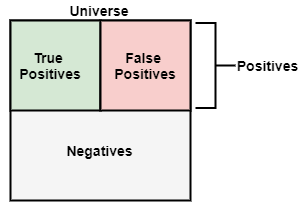
\includegraphics[width=0.3\textwidth]{thesis/figures/bloom-universe.png}
            \caption{Partitioning the Universe using a bloom filter}
            \end{figure}
            
            \newpage
            {\bf Reconstruction Errors}:
            \begin{enumerate}[label=(\alph*)]
            
            \item {\bf Indices from $P-S$ are falsely assigned to non-zero values.} \\
            {\it Those indices are normally destined by the underlying sparsification method to be assigned to zero values during the decoding process. 
            However now, when a "false positive" index is selected by a policy $\mathcal{P}$, it will be mapped to a non-zero value.
            This is a direct consequence of the occurrence of false positive responses and the specific formulation of the decompression algorithm.}
            
            \item {\bf The values that indices from $P-S$ are mapped to belong in $\{\tilde{g}[i]\}_{i\in S}$. } \\
            {\it In practice, this means that not only those indices are assigned to non-zero values, as discussed in item (a) but they also take over values from $\{\tilde{g}[i]\}_{i\in S}$ which causes the disruption of the mapping process $\mathcal{M}$ and leads to the next type of errors.}
            
            \item {\bf "True Positive Indices" may not be assigned to their designated values.} \\
            {\it This is an immediate consequence of (a) and (b).
            All those indices from $\tilde{S} \cap S$ that are visited after we encounter the first falsely selected index, are not assigned to the correct values from $\{\tilde{g}[i]\}_{i\in S}$, as those were taken over by other, precedent indices.}
            
            \end{enumerate}
            
            We observe that there is a strong correlation between those three types of errors and while there is no way to fully mitigate (a) without dramatically increasing the size $m$ of the Bloom Filter, we can probably remedy (b) and (c), as we will discuss in a later chapter.
            One possible direction of this work would be to study these reconstruction errors with respect to the properties of the Bloom Filters, understand their impact in training and examine whether convergence can be guaranteed even under their presence.
            Whereas there have been some experimental results depicting that training cannot tolerate in practice that kind of rearrangements in the gradient components, we have selected not to focus on this particular direction. 
            Instead, our aim was to improve the bloom filters approach by either integrating ideas that will reduce the false positive rate while keeping the bloom filter size small or by trying to tackle the above reconstruction errors.


    % \newpage

    \section{Policies for Choosing Indices}
    We have mentioned about the policy $\cP$ in the previous section. 
    Formally speaking, a policy $\mathcal{P}$ is a process that receives a set $P$ as input and yields a subset $\tilde{S}$ of $P$ that contains $r$ elements as output.
    Note that,  $r=\|\tilde{g}\|_0$ is the number of sparsified gradient values and thus, the number of elements in $S$ and
    $P$ is the set of indices corresponding to the bloom filter's non-negative responses.
      
    The notion of policies is an integral part of the encoding and decoding algorithms in our bloom filter approach.
    A poor policy will have a significantly negative impact on the gradients reconstruction and therefore, in the overall training process.
    We will introduce a formal way for evaluating different policies under some fixed bloom filter properties in the next sections 
    but first, we will describe some policies that we developed and used for our experiments.
    
    \begin{figure}[h]
    \centering
    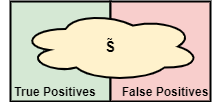
\includegraphics[width=0.3\textwidth]{thesis/figures/policy.png}
    \caption{Set \tilde{S} of selected indices given a policy \mathcal{P}}
    \end{figure}
    
        % \newpage
        \subsection{Leftmost-r}
            We order the indices in $P$ in an increasing order and we choose the first $r$ to be our subset $\tilde{S}$. 
            We call it leftmost-r because the first $r$ elements in the sorted $P$ are its $r$ leftmost elements.
            Note that, the selection of such a policy is not as random as it may seems.
            Remember that during the decoding phase, we need to make queries for all the elements of the universe $U$ in order to determine all the non-negative bloom filter responses and create $P$. 
            The most straightforward way to implement this, is to iterate over $U$ in an increasing order.
            This policy implies that we create $\tilde{S}$ on the fly while still iterating and posing queries.
            This algorithm is relatively faster compared to other policies because in practice, one does not need to explore the full universe in order to retrieve $\tilde{S}$.
            They can simply stop as soon as they collect the first $r$ "false positive" elements.
            However, this still is considered to be a naive approach as it ignores a lot of actual implementation aspects that could help us decrease the selection of indices corresponding to false positive responses. 
            
     
        \subsection{Random-r}
            We create $\tilde{S}$ by picking randomly $r$ indices from $P$.
            Note that, the previous policy could be considered as a sub-case of Random-r. Whereas this method does not tend to favor smaller indices, it still does not fully exploit the specific characteristics of our bloom filter setting.
        
        \subsection{Conflict Sets}
            In order to devise a better policy, we first need to realize some of the characteristics that distinguish our bloom filter setting from its other more common applications.
            Notice that, in our case, the set of elements that comprise the universe $U$ of the bloom filter is finite and those elements are also known to us.
            The fact that we strategically query every single element of $U$, as part of the decompression process, is crucial.
            It enables us to consider knowledge related to the bloom filter's construction process and use it in order to make better probabilistic choices of indices while creating $\tilde{S}$.
            That is, indices that are more probable to correspond to true positive bloom filter responses.
            We achieve that by organizing the elements inside $P$ in a number of smaller sets that share some interesting properties and we call them as "conflict sets".
            
            As the title suggests, a conflict set comprises elements that correspond to non-negative bloom filter responses and reside at the same bit location inside the bloom filter. In the context of bloom filters, we say that those elements create a conflict with one another.
            
            % \newpage
            Formally speaking, we define a conflict set as:
            \begin{flushleft}
            % \setlength{\parindent}{20ex}
            $ \mathcal{C}_j = \{x \mid x \in P\ and\ \mathcal{H}_i(x)=j\ for\ at\ least\ one\ i=1,2,\cdots,k \}$, 
            
            where $\mathcal{H}_i(x)$ is the bit location inside the filter as it is indicated by the $h_i$ hash function.
            \end{flushleft}
            
            % $ \mathcal{C}_j^i = \{x \mid \in P$ and $ h_i(x)=j \} $
            % let $\mathcal{H}$ = $\{h_i \mid i=1,2,\cdots,k\}$
            % a $h \in \{h[i]\}_{i\in \{1,2,\cdots,k\} }$\} $
            % $\{\forall i,j \in \mathcal{C} h(i)=h(j)$

            It is readily seen that the following rules apply:
            \begin{enumerate}[label=(\alph*)]
            \item Every conflict set contains at least one element that corresponds to a true positive bloom filter response.
            \item As an immediate consequence of $(a)$, there are at most $r*k$ different conflict sets.
            \item The union $\bigcup C_{j}$ of all $j$ equals to $P$. 
            Notice that, for $k=1,\ i \neq j \implies C_i \cap C_j=0$.
            \end{enumerate}

            Now, we can leverage this information and devise a heuristic strategy for repeatedly drawing indices out of the conflict sets until we create $\tilde{S}$.
            
            We develop such a method by satisfying the following objectives:
            \begin{itemize}
                \item During the selection of indices we should prioritize drawing from conflict sets for which we are certain that $(a)$ still holds.
                It is important to note that, as we start to draw elements, our ability to know for sure whether a conflict set still contains true positives is very limited.
                At each given moment, we can be sure that $(a)$ holds only for those sets $C_j$ for which $C_j \cap \tilde{S}=0$. 
                That is sets strictly containing elements that have not been yet selected.
                In other words, when we select a new index, we are bound to assume that it is the true positive that causes the conflict sets in which it appears to satisfy $(a)$. 
                As far as we know, in its absence, those conflict sets may or may not contain true positives anymore.
                
                \item If more than one conflict sets have been favored because of the above reason, then we prioritize those having a smaller size. 
                Assuming that we have a good enough set of hash functions that distribute elements uniformly inside the bloom filter, we should not observe extreme differences between the sizes of conflict sets. 
                However, given our limited knowledge regarding the actual distribution of true positives inside the conflict sets and in order to maintain the computational complexity of this method as small as possible, we assume that true positives are also uniformly dispersed across the sets and therefore, the probability of drawing a true positive out of a smaller set should be higher.
            \end{itemize}
            
            The formulation of those objectives was mostly driven by one particular observation. It is often the case that many of the true positive elements can be actually inferred rather than guessed. 
            This happens because some of the conflict sets may be singletons i.e. contain only one element.
            As an immediate consequence of $(a)$, we can infer that the elements of those unit sets are true positives and thus, we can automatically add them in $\tilde{S}$.
            
            Finally, if we have not finished with the construction of $\tilde{S}$ and we have no reason to prioritize any conflict sets due to our lack of information about whether they still satisfy $(a)$ or not, we may as well interchange between them and randomly pick the remaining number of indices.

            What makes this policy more sophisticated than the ones mentioned earlier, is mostly its ability to infer some of the true positives in case we have singleton sets.
            It is also unbiased in the sense that it does not favor particular indices, like leftmost-r does.
            
            \newpage
            Imagine the following example where we consider $k=1$ for simplicity:
            \begin{itemize}
                \item Let $P = \{{\bf 0}, 1, {\bf 5}, {\bf 3}, {\bf 4}, 6, {\bf 8}, 9\}$, where the elements in bold are the true positives.
                \item Now, let $P$ be organized in conflict sets as follows:
                $\{\{{\bf 0},1, {\bf 5}\}, \{{\bf 3}\}, \{{\bf 4},9\}, \{{\bf 8},6\}\}$.
                Notice that, now that $k=1$, an element cannot exist in two different conflict sets.
                    
                \item All of those conflict sets contain at least one true positive.
                Thus, it is only logical to not exclude any of them from the selection process.
                We prioritize the conflict set with the smallest size which in this case is a singleton. 
                We select the element $3$ for which we can also infer that it is a true positive.
                
                \item As we already said, $3$ is not included in any other set, now that $k=1$, so all the remaining conflict sets are still eligible for the next selection. 
                Similarly, between 
                \{{\bf 0},1, {\bf 5}\}, \{{\bf 4},9\} and \{{\bf 8},6\} we give less priority to \{{\bf 0},1, {\bf 5}\} due to its bigger size.
                Let us say that we draw the element $4$ from the set \{{\bf 4},9\}. Notice that, even though $4$ is actually a true positive, we have no way of knowing that. We are no longer sure whether \{9\} contains a true positive or not, so we will no longer prioritize this set.
                \item Suppose that the next selection is the element $6$ from the set \{{\bf 8},6\}. Still, we are not aware that we selected a false positive index, therefore, we are bound to stop prioritizing  \{{\bf 8}\} as well, even though it contains a true positive.
                \item \{{\bf 0},1, {\bf 5}\} is the last set, for which we surely now that $(a)$ still holds. Suppose that we draw the element $0$ which happens to be a true positive. 
                \item So far, we have $\tilde{S}=\{{\bf 3},{\bf 4},6, {\bf 0}\}$.
                $P$ is now organized as follows: \{\{1, {\bf 5}\}, \{\}, \{9\}, \{{\bf 8}\}\} and there is one more index that we need to select.
                As we discussed, we could now arbitrarily choose between the remaining conflict sets or develop a more complex strategy by taking into account the sizes of those sets.
                
                \end{itemize}
                
                Notice that, the probability of drawing $r$ true positives from $P$ using the Random-r policy would be $1/\binom{8}{5} = 1/56$, whereas now it is:
                $1/48$.
                
                The Conflict Sets policy could be characterized as a generalized case of Random-r. 
                Consider the scenario where we have a terrible set of hash functions all mapping the elements in $P$ to the same bit location. $P$ would now be organized as one, big conflict set from which we would randomly pick values. 
                This is equivalent to what we do in Random-r policy.

    \section{Policy Errors Rate}
        Although the false positive rate is useful as a metric for evaluating a bloom filter's performance, we can see that the actual rate of selecting false positive indices during the decompression process also depends on the underlying policy.
        Imagine we have a bloom filter that produces a large number of false positive responses but we have somehow constructed an ideal policy than can successfully identify and select only the true positives.
        Then the false positive selection rate would be $0$ whereas the false positive rate of the bloom filter would be much greater.
        We call this new metric policy errors rate and we use it alongside the false positive rate metric in order to evaluate the performance of the decompression process.
        More specifically, we define the policy errors rate as the number of false positive indices selected over the total number of selections that took place.
        Note that, this metric strongly depends on the FPR metric as the greater the later is the harder it is for the underlying policy to distinguish and select the true positives.

    \section{Second Bloom Filter built on false positives}
        Another idea that aims to reduce the false positive rate is that of using a second bloom filter. 
        The first bloom filter will be built on $S$ as per normal and the second one will be used to represent the set $P-S$ of elements corresponding to false positive responses. 
        Now, we modify the decompression process by also consulting the second bloom filter when the first one yields a positive response for a given element.
        That is, we pass the set $P$ through a second phase of querying with the hope that many of its true positive elements will be identified by the second bloom filter.
        More specifically, if the second bloom filter returns a negative response for an element $x \in P$ then we know with complete certainty that $x$ does {\bf not} belong in $P-S$, thus it is a true positive.
        Otherwise, the status of $x$ continues to be unknown.
        The newly identified true positives will then be inserted to $\tilde{S}$.
        
        Let $P_2 \subset P$ be the set of the remaining indices of $P$ after we prune it with the help of the second bloom filter.
        The rest of the decompression algorithm remains the same with the only difference being that the policy $\mathcal{P}$ will now select indices from $P2$ instead of $P$ as many times as necessary in order to have a total of $r$ elements in $\tilde{S}$.
        
        \begin{figure}[h]
        \centering
        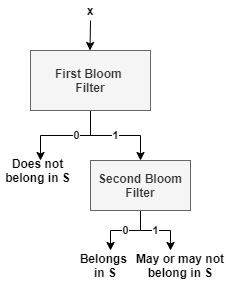
\includegraphics[width=0.3\textwidth]{thesis/figures/second-bloom.png}
        \caption{Second Bloom Filter Built on False Positives}
        \end{figure}

        An obvious disadvantage of this idea is that we must now communicate not one but two bloom filters.
        Remember that, what makes the bloom filter approach appealing compared to some other lossless encoding methods like run length encoding is its space efficiency.
        The additional space needed to store the second bloom filter might make the overall usage of this lossy encoding method worthless.

    \section{False Positives Aware Compression}
        All these ideas aim to improve the bloom filters' performance.
        However, even if we focus on reducing the FPR by employing more sophisticated versions of bloom filters there is no guarantee that we will eliminate the occurrence of false positives. 
        Also, decreasing the FPR to the point that false positives no longer have real impact in training will probably increase the bloom filters' size which is another important constraint in our application.
        
        As we already discussed, the decompression process is  sensitive, in practice, to the occurrence of false positives as they tend to deteriorate training.
        We described three different types of reconstruction errors and we suggested that there is a way to mitigate some of those.
        More specifically, we will now present an idea that aims to tackle the errors $(b)$ and $(c)$, meaning we will try to avoid having re-arrangements of the reconstructed gradient components with respect to their true positions under the presence of false positives.
        
        Remember that, in our very special setting, we have the luxury of knowing while encoding a gradient both the set of items that comprise the bloom filter's universe and the exact queries that are going to be posed during the decompression process.
        As long as the policy $\mathcal{P}$ is a deterministic process that can be reproduced, we can also know at construction time the set $\tilde{S}$ that is going to be generated during the decoding phase.
        
        This enables the compression process to appropriately modify the sparsified gradient that is to be communicated as part of the message in a way that will smooth out the decoding and eliminate disruption.
        More specifically, while compressing a gradient we can
        know beforehand all the errors that will occur during the decompression phase by simply executing the decompress algorithm on the encoded gradient.
        This way we can detect all bloom filter's non-negative responses and more importantly we can acquire the set $\tilde{S}$ of the future selected indices that are going to be paired with the values from $\{\tilde{g}[i]\}_{i\in S}$.
        This knowledge allows us to replace some of these gradient components with others so that all the final values communicated over the network will be the ones that actually correspond to the indices from $\tilde{S}$.
        
        Remember that, the values in $\{\tilde{g}[i]\}_{i\in S}$ are selected by the given sparsification method.
        Replacing some of those values with others, selected from the initial gradient, is like tampering with the underlying sparsification method.
        
        We demonstrate this idea using the following example:
        \begin{itemize}
            \item Let $\{{\bf 20}, 14, 13, {\bf 22}, {\bf 21}, 15, 19, 11, {\bf 28}, 10\}$ be the initial gradient, where the elements in bold are the values selected by the underlying sparsification method (notice that here we are using the Top-r sparsification method).
            So, we have $\{\tilde{g}[i]\}_{i\in S} = \{{\bf 20, 22, 21, 28}\}$ and it follows that $S=\{0,3,4,8\}$
    
            \item Now, let $P=\{{\bf 0}, 1, {\bf 3}, {\bf 4}, 6, {\bf 8}, 9\}$, where the elements in bold are the true positives and 
            let $\tilde{S}=\{{\bf 0}, {\bf 3}, 6, 9\}$ be the set of indices selected using a given policy $\mathcal{P}$.
            Notice that, the policy errors rate in this case is equal to $0.5$, meaning that out of the $4$ true positive indices in $S$ we managed to "guess" right only $2$ of them.

            \item The message that will be sent to the workers comprises the values in $\{\tilde{g}[i]\}_{i\in S}$ as well as the bloom filter that represents $S$.
            However, being aware of the false positives that are going to occur during the decompression process, we can now remove the values in $\{\tilde{g}[i]\}_{i\in S}$ that correspond to the true positive indices that are not going to be selected. 
            In their place, we are going to add those gradient components that actually correspond to the false positive indices that are falsely selected.
            In other words, we now send $\{\tilde{g}[i]\}_{i\in \tilde{S}}$ instead of $\{\tilde{g}[i]\}_{i\in S}$.
            That is, $\{{\bf 20, 22}, 19, 18\}$.
            Notice that, without the false positive aware compression, the decoded gradient would be: $\{{\bf 20}, 0, 0, {\bf 22}, 0, 0, {\bf 21}, 0, 0, {\bf 28}\}$, 
            whereas now it is: $\{{\bf 20}, 0, 0, {\bf 22}, 0, 0, 19, 0, 0, 10\}$.
            
        \end{itemize}
        
        The obvious drawback of this solution is that for every false positive bloom filter response we defy the underlying sparsification method by sacrificing one of its gradient component choices.
        Note that, in the absence of false positives, this method is equivalent to the given sparsification method (e.g. Top-r) whereas it turns more and more into the Random-r method as false positives start to occur.
        In this sense, we could say that the false positive aware compression is strongly coupled with the given sparsification method and thus, can be considered as a hybrid sparsification method itself.
